\documentclass{standalone}
\usepackage{tikz}
\begin{document}
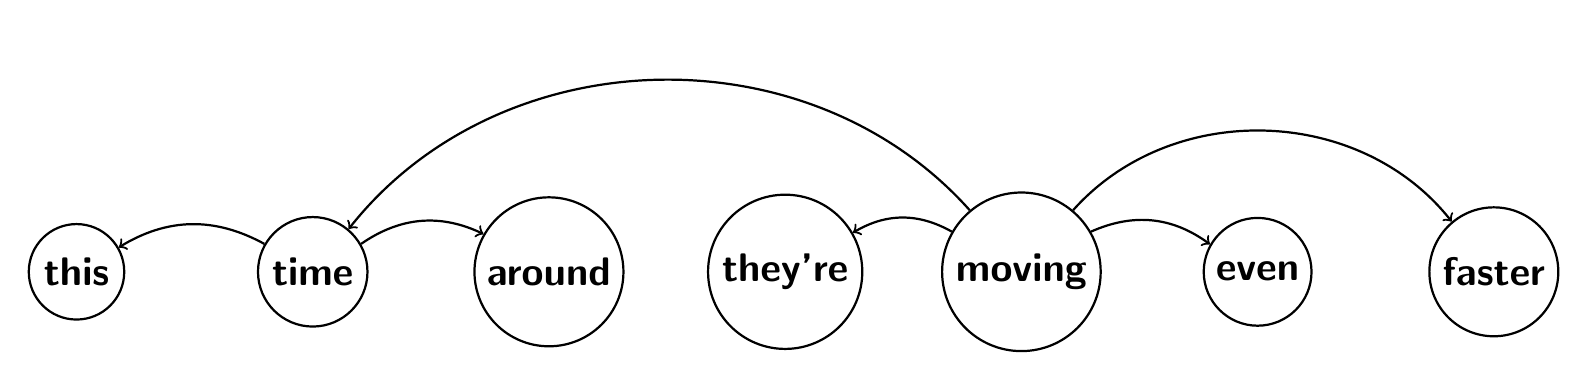
\begin{tikzpicture}[->, node distance=3cm, every loop/.style={},
                    thick,main node/.style={circle,draw,font=\sffamily\Large\bfseries}]

  \node[main node]   (this)   {this};
  \node[main node]   (time)   [right of=this] {time};
  \node[main node]   (around) [right of=time] {around};
  \node[main node]   (they're)[right of=around] {they're};
  \node[main node]   (moving) [right of=they're] {moving};
  \node[main node]   (even)   [right of=moving] {even};
  \node[main node]   (faster) [right of=even] {faster};

  \path[] (moving) [bend right] edge (they're);
  \path[] (moving) [bend left] edge (even);
  \path[] (moving) [bend left=50] edge (faster);

  \path[] (moving) [bend right=50] edge (time);
  \path[] (time) [bend left] edge (around);
  \path[] (time) [bend right] edge (this);
\end{tikzpicture}
\end{document}